\documentclass[border=20pt]{standalone}
\renewcommand\familydefault{\sfdefault} % Default family: serif 
%\usepackage[usenames,dvipsnames]{xcolor}
\usepackage[x11names]{xcolor}
\usepackage{tikz}
\usepackage{soulutf8}
\usetikzlibrary{arrows,fit,positioning,shapes,calc}

%\definecolor{WIRE}{HTML}{002FA7} % Klein Blue
\usepackage[normalem]{ulem}

\tikzstyle{every entity} = []
\tikzstyle{every weak entity} = []
\tikzstyle{every attribute} = []
\tikzstyle{every relationship} = []
\tikzstyle{every link} = []
\tikzstyle{every isa} = []

\tikzstyle{link} = [>=triangle 60, draw, thick, every link]

\tikzstyle{total} = [link, double, double distance=3pt]

\tikzstyle{entity} = [rectangle, draw, black, very thick,
minimum width=6em, minimum height=3em,
every entity]

\tikzstyle{weak entity} = [entity, double, double distance=2pt,
every weak entity]

\tikzstyle{attribute} = [ellipse, draw, black, very thick,
minimum width=5em, minimum height=2em,
every attribute]

%\tikzstyle{key attribute} = [attribute, font=\bfseries]

\tikzstyle{multi attribute} = [attribute, double, double distance=2pt]

\tikzstyle{derived attribute} = [attribute, dashed]

%\tikzstyle{discriminator} = [attribute, font=\itshape]

\tikzstyle{relationship} = [diamond, draw, black, very thick,
minimum width=2em, aspect=1,
every relationship]

\tikzstyle{ident relationship} = [relationship, double, double distance=2pt]

\tikzstyle{isa} = [isosceles triangle, isosceles triangle apex angle=60,
shape border rotate=-90,
draw, black, very thick, minimum size=3em,
every isa]

% for text un key attributes
\newcommand{\key}[1]{\underline{#1}}
\newcommand{\pkey}[1]{\dashuline{#1}}

% for text in discriminator attributes
\def\discriminator{\bgroup 
	\ifdim\ULdepth=\maxdimen  % Set depth based on font, if not set already
	\settodepth\ULdepth{(j}\advance\ULdepth.4pt\fi
	\markoverwith{\kern.15em
		\vtop{\kern\ULdepth \hrule width .3em}%
		\kern.15em}\ULon}

%%


\definecolor{MediumPurple1}{rgb}{0.58, 0.44, 0.86}
\definecolor{Chartreuse2}{rgb}{0.5, 1.0, 0.0}
\tikzset{every entity/.style={draw=orange, fill=orange!20}}
\tikzset{every attribute/.style={draw=MediumPurple1, fill=MediumPurple1!20}}
\tikzset{every relationship/.style={draw=Chartreuse2, fill=Chartreuse2!20}}

%% Variable for participation constraint
\newcommand{\cM}{\mathrm{M}}
\newcommand{\cN}{\mathrm{N}}
\newcommand{\cO}{\mathrm{O}}
\newcommand{\cP}{\mathrm{P}}

\begin{document}


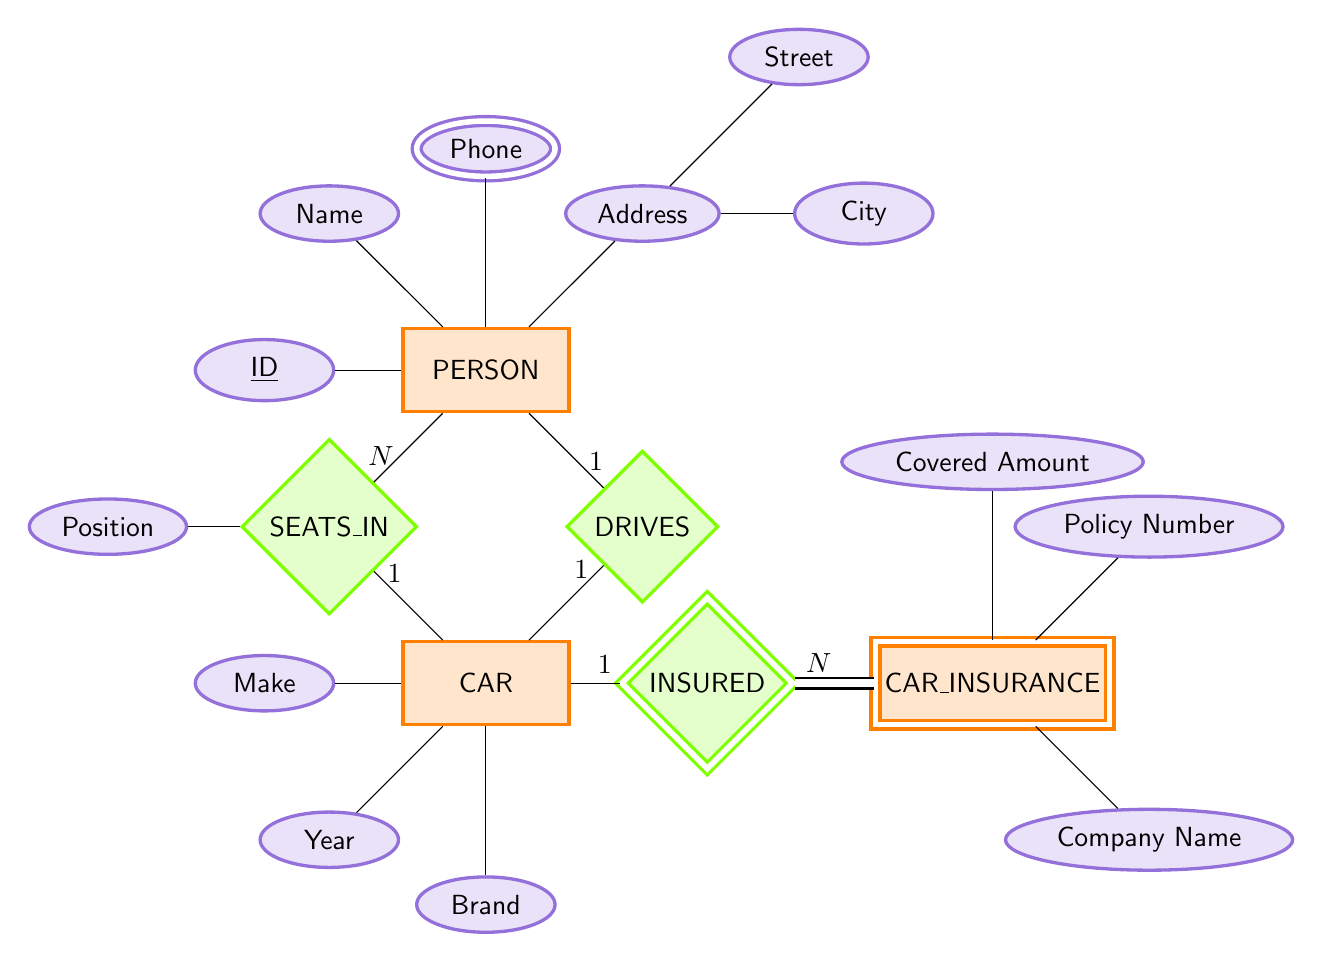
\begin{tikzpicture}[node distance=8em]
	\node[entity] (person) {PERSON};
	\node[attribute] (pid) [left of=person] {\key{ID}} edge (person);
	\node[attribute] (name) [above left of=person] {Name} edge (person);
	\node[multi attribute] (phone) [above of=person] {Phone} edge (person);
	\node[attribute] (address) [above right of=person] {Address} edge (person);
	\node[attribute] (street) [above right of=address] {Street} edge (address);
	\node[attribute] (city) [right of=address] {City} edge (address);
	%\node[derived attribute] (age) [right of=person] {Age} edge (person);

	\node[relationship] (drives) [below right of=person] {DRIVES} edge node[above, pos=0.1] {$1$} (person);
	\node[entity] (car) [below left of=drives] {CAR} edge node[above, pos=0.7] {$1$} (drives);
	\node[attribute] (make) [left of=car] {Make} edge (car);
	\node[attribute] (year) [below left of =car] {Year} edge (car);
	\node[attribute] (brand) [below of =car] {Brand} edge (car);

	\node[relationship] (seats) [below left of=person] {SEATS\_IN} edge node[above, pos=0.1] {$N$} (person);
	\draw (seats) edge node[above, pos=0.3] {$1$} (car);
	\node[attribute] (position) [left of=seats] {Position} edge (seats);

	\node[ident relationship] (insured) [right of=car] {INSURED} edge node[above, pos=0.3] {$1$} (car);
	\node[weak entity] (insurance) [right = 1cm of insured] {CAR\_INSURANCE} edge[total] node[above, pos=0.7] {$N$} (insured);
	\node[attribute] (amount) [above of =insurance] {Covered Amount} edge (insurance);
	\node[attribute] (policy) [above right of =insurance] {Policy Number} edge (insurance);
	\node[attribute] (company) [below right of =insurance] {Company Name} edge (insurance);
\end{tikzpicture}

\end{document}
